\documentclass[spanish]{beamer}
%
\include{conf/preconfig}
\include{conf/packages}
\include{conf/config}
\include{beamerconf}
%
%\usetheme{Antibes}
\usetheme{Warsaw}
\usecolortheme{orchid}
%
%
\title{Identificación de edificios y monumentos a partir de fotografías tomadas
con dispositivos móviles}
\author{Esteban C. Fornal \and Christian N. Pfarher \and Mauro J. Torrez}
\date{\today}
%
\begin{document}
%
\frame{\titlepage}
%
%%%%%%%%%%%%%%%%%%%%%%%%%%%%%%%%%%%%%%%%%%%%%%%%%%%%%%%%%
\section{Objetivo}
\begin{frame}
  \frametitle{Objetivo}
  Identificar edificios y monumentos a partir de fotografías
\end{frame}
%
%%%%%%%%%%%%%%%%%%%%%%%%%%%%%%%%%%%%%%%%%%%%%%%%%%%%%%%%%
\section{Herramientas utilizadas}
\begin{frame}{Herramientas}
  \begin{itemize}
  \item<1-> Transformada de Hough
  \item<2-> Histograma
  \end{itemize}
\end{frame}
%
%%%%%%%%%%%%%%%%%%%%%%%%%%%%%%%%%%%%%%%%%%%%%%%%%%%%%%%%%
\section{Técnicas utilizadas}
%
\subsection{Transformada de Hough}
\begin{frame}{Transformada de Hough}
\begin{center}
  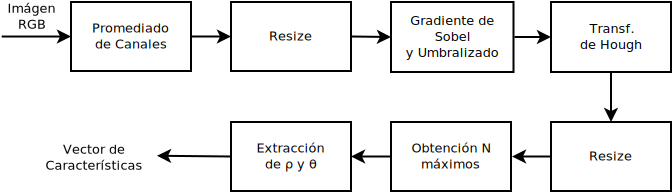
\includegraphics[width=9cm]{../diagramas/procesohough}
\end{center}
\begin{itemize}
\item[]\begin{center}
  \begin{equation*}
    \label{umbral}
    f(I)=
    \begin{cases}
      0, & I\leq U\\
      255, & I > U
    \end{cases}
  \end{equation*}
\end {center}
\item 60 características
\end{itemize}
\end{frame}
%
\subsection{Estadísticas del Histograma}
\begin{frame}{Estadísticas del Histograma}
 \begin{center}
   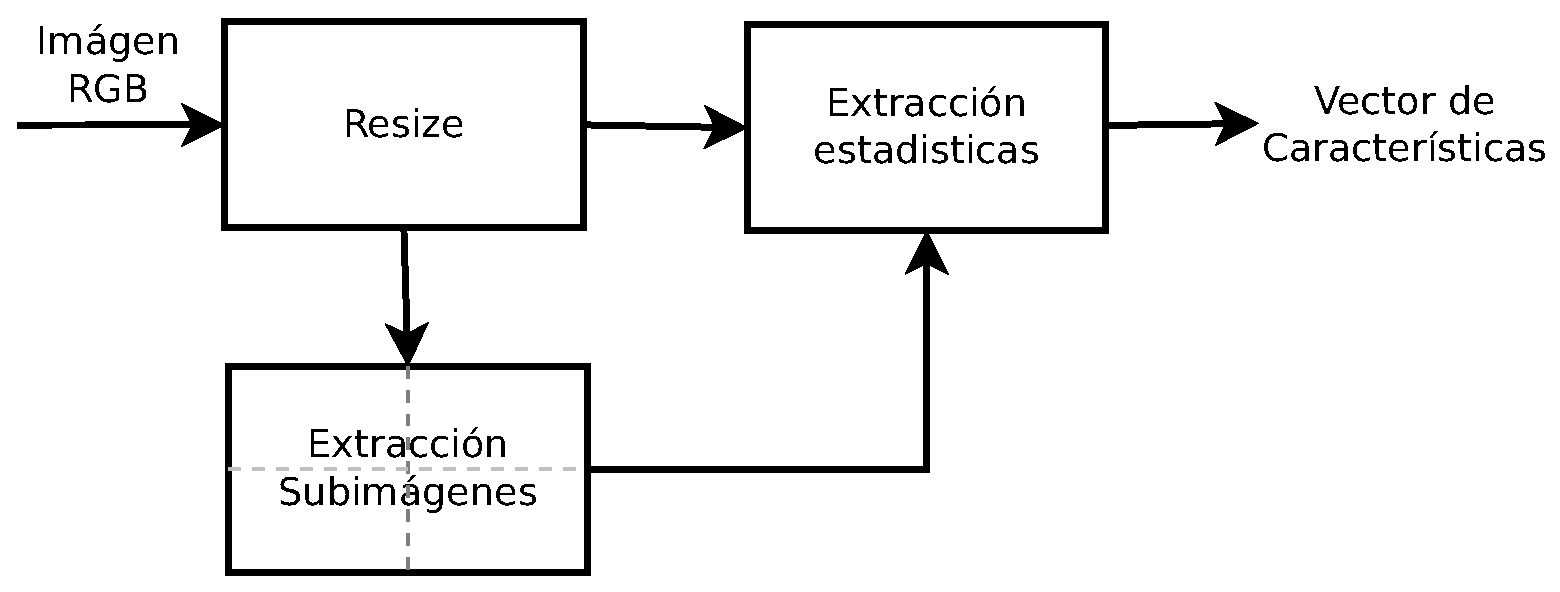
\includegraphics[width=9cm]{../diagramas/procesoestadisticas}
 \end{center}
 \begin{itemize}
 \item 45 características
 \end{itemize}
\end{frame}
%
%%%%%%%%%%%%%%%%%%%%%%%%%%%%%%%%%%%%%%%%%%%%%%%%%%%%%%%%%
\section{Método}
%
\subsection{Entrenamiento}
\begin{frame}{Entrenamiento}
  \begin{itemize}
  \item Etiquetado de imágenes
  \item Generación de prototipos
  \end{itemize}
\end{frame}
%
\subsection{Clasificación}
\begin{frame}{Clasificación}
  \begin{itemize}
  \item Error cuadrático medio:
\begin{equation}
  p_{\T{ganador}}=\arg \min_i\left\{ \frac{1}{\sum N_j}
                \sum_{j=1}^K\sum_{n=1}^{N_j}(t_j[n]-p_{ij}[n])^2\right\}
\end{equation}
\item Obtención de la Clase
  \end{itemize}
\end{frame}
%
%%%%%%%%%%%%%%%%%%%%%%%%%%%%%%%%%%%%%%%%%%%%%%%%%%%%%%%%%
\section{Pruebas}
%
\subsection{Armado Base de Datos}
\begin{frame}{Armado Base de Datos}
  \begin{itemize}
  \item Imágenes de 640x480
  \item Obtenidas con celular
  \item Diurnas y nocturnas
  \end{itemize}
\end{frame}
%
\subsection{Conjunto de Imágenes}
\begin{frame}{Clases}
  \includegraphics[width=10cm]{img/mosaico.png}
\end{frame}
%
\begin{frame}{Imágenes de prueba}
  \includegraphics[width=10cm]{img/pruebas.png}
\end{frame}
%
\subsection{Sólo con técnica de T. de Hough}
\begin{frame}{Sólo con la técnica de Hough}
  Determinación de umbral y cantidad de máximos a utilizar
  \begin{center}
    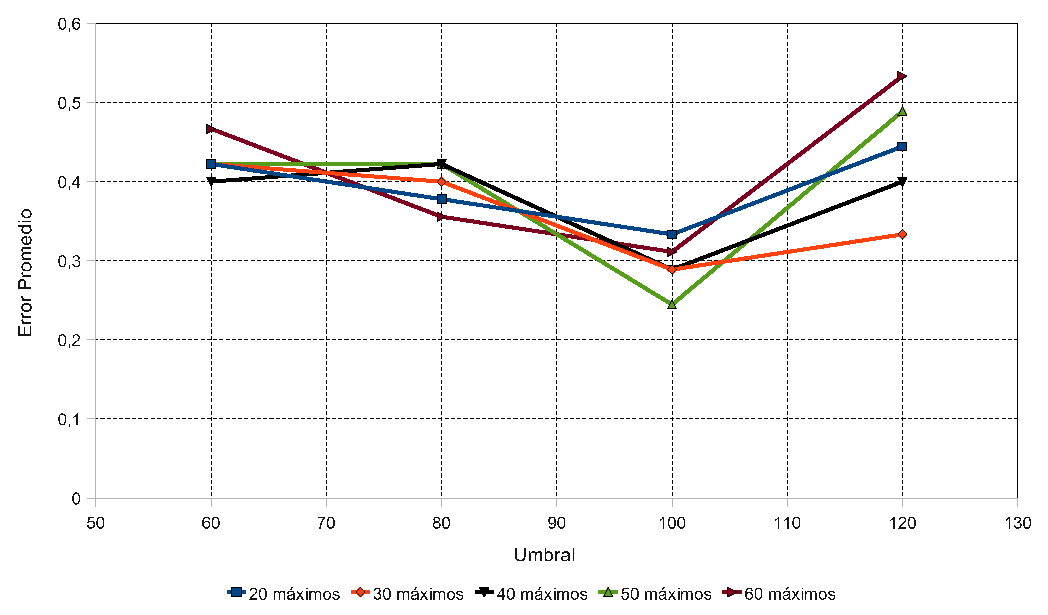
\includegraphics[width=9cm]{../diagramas/estadistica_noche_iguales}
  \end{center}
\end{frame}
%
\subsection{Sólo con técnica de histograma}
\begin{frame}{Sólo con la técnica de histograma}
\end{frame}
%
\subsection{Hough+Histogramas}
\begin{frame}{Hough+Histogramas}
  \begin{itemize}
  \item Igual ponderación
  \end{itemize}
\end{frame}
%
\subsection{Cómo se hicieron?}
\begin{frame}{Procedimiento}
  \begin{center}
%    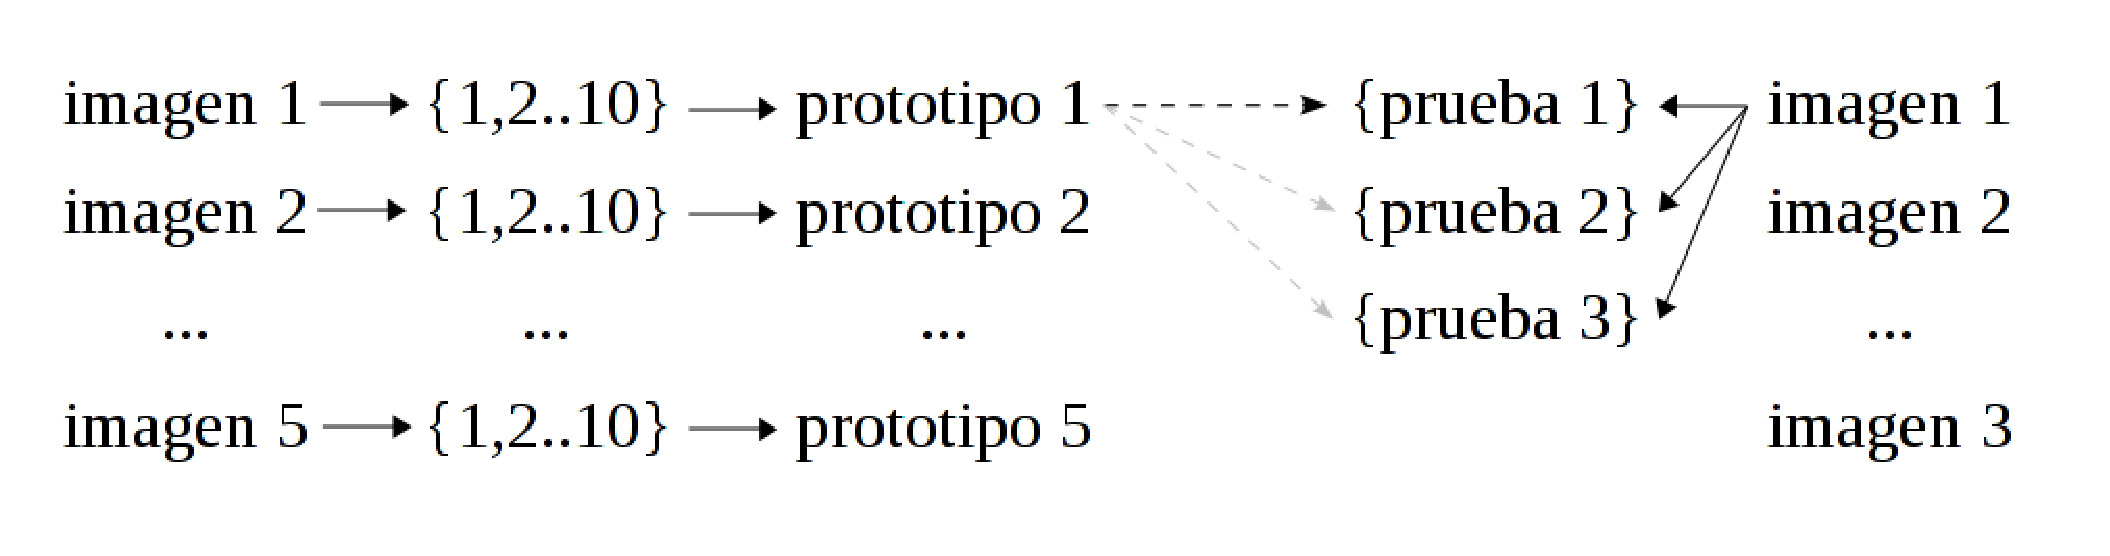
\includegraphics[width=11cm]{../diagramas/proceso_pruebas}
  \end{center}
\end{frame}
%
%%%%%%%%%%%%%%%%%%%%%%%%%%%%%%%%%%%%%%%%%%%%%%%%%%%%%%%%%
\section{Resultados}
\begin{frame}{Resultados}
  Se considera la tasa de error según:
  \begin{equation*}
    E_{\%}=100\cdot\frac{\T{número de errores}}{\T{número de pruebas}},
  \end{equation*}

  Tasas de error para las técnicas de extracción de características
  \begin{center}\begin{tabular}{ccc}
      \hline \emph{{Técnica}} & \emph{5 etiquetas} & \emph{15 etiquetas}\\
      \hline Histogramas & 0\% & 0\%\\
      \hline Hough & 35.5\% & 60.43\%\\
      \hline Ambas & 2.22\% & 4.17\%\\
      \hline
  \end{tabular}\end{center}
\end{frame}
%
%%%%%%%%%%%%%%%%%%%%%%%%%%%%%%%%%%%%%%%%%%%%%%%%%%%%%%%%%
\section{Conclusiones}
\begin{frame}{Conclusiones}
  \begin{itemize}
  \item Satisfactorio coinciderando restricciones
  \item Optimización para dispositivos móviles
  \item Preprocesamiento de la imágen
  \end{itemize}
\end{frame}
%
%%%%%%%%%%%%%%%%%%%%%%%%%%%%%%%%%%%%%%%%%%%%%%%%%%%%%%%%%
\section{Trabajos futuros}
\begin{frame}{Trabajos futuros}
  \begin{itemize}
  \item Preprocesamiento
  \item Filtrado homomórfico
  \item Warping
  \item Costo computacional
  \end{itemize}
\end{frame}
%%%%%%%%%%%%%%%%%%%%%%%%%%%%%%%%%%%%%%%%%%%%%%%%%%%%%%%%%
\begin{frame}{}
  \begin{itemize}
  \item<1-2> ¿Preguntas?
  \item<2-> ¡Muchas gracias!
  \end{itemize}
\end{frame}
\end{document}
